\documentclass{article}

% ── Track selection ──────────────────────────────────────────────────────────
% Submission (double-blind, default):
\usepackage[preprint]{neurips_2026}
% Camera-ready (after acceptance):
% \usepackage[main, final]{neurips_2026}

% ── Standard packages ────────────────────────────────────────────────────────
\usepackage[utf8]{inputenc}
\usepackage[T1]{fontenc}
\usepackage{hyperref}
\usepackage{url}
\usepackage{booktabs}
\usepackage{amsfonts}
\usepackage{amsmath}
\usepackage{amssymb}
\usepackage{xcolor}
\usepackage{graphicx}
\usepackage{enumitem}

\raggedbottom
\hbadness=4000

% ── Notation macros ──────────────────────────────────────────────────────────
\newcommand{\calF}{\mathcal{F}}
\newcommand{\calD}{\mathcal{D}}
\newcommand{\calC}{\mathcal{C}}
\newcommand{\calL}{\mathcal{L}}
\newcommand{\calA}{\mathcal{A}}
\newcommand{\RR}{\mathbb{R}}
\newcommand{\EE}{\mathbb{E}}
\newcommand{\PP}{\mathbb{P}}
\newcommand{\Nclients}{K}                % number of clients
\newcommand{\Nrounds}{T}                 % communication rounds
\newcommand{\params}{\boldsymbol{\theta}}% model parameters
\newcommand{\grad}{\nabla}
\newcommand{\EOpp}{\mathrm{EO}}          % Equal Opportunity
\newcommand{\DP}{\mathrm{DP}}            % Demographic Parity
\newcommand{\DEOpp}{\Delta\mathrm{EO}}   % Delta Equal Opportunity

% ─────────────────────────────────────────────────────────────────────────────
\title{Fairness by Intervention: Client-Side Fairness Strategies\\
  and Server Auditing Protocols in Federated Learning}

\author{%
  \textbf{Kshitish Kiran Madbhavi}\\
  \textit{Indian Institute of Technology Gandhinagar}\\
  \texttt{kshitish.madbhavi@iitgn.ac.in}
}

% ─────────────────────────────────────────────────────────────────────────────
\begin{document}

\maketitle

% ── Abstract ─────────────────────────────────────────────────────────────────
\begin{abstract}
Federated learning (FL) can amplify demographic disparity under
client-level heterogeneity, but fairness-targeted local interventions
can also alter this behavior in non-trivial ways.
We present a controlled empirical study of five client-side fairness
interventions (I$_1$--I$_5$, legacy labels A$_1$--A$_5$) and five
server-side auditing/stabilization protocols
(P$_1$--P$_5$, legacy labels D$_1$--D$_5$).
The evaluation uses UTKFace gender classification with
\texttt{race\_bin} as the protected attribute, ResNet18, 20 clients,
8 sampled clients per round, 30 rounds, three data regimes
(IID, Dirichlet-$\alpha{=}0.5$, strict non-IID), and three optimizers
(SGD, AdamW, FedProx).
We execute the full 189-configuration profile end-to-end
(single seed: 42) and report descriptive statistics.
The central finding is that optimizer choice dominates
intervention-protocol outcomes: in intervention+protocol runs, AdamW
reaches mean accuracy 0.7730,
while SGD and FedProx collapse to 0.4545 and 0.4543, respectively.
Among intervention-only settings, I$_4$ is most disruptive on average
($\Delta$Acc $=-0.1500$ vs matched baselines).
No protocol is uniformly best: P$_4$ attains the highest mean accuracy
(0.5758) but also the largest mean equalized-odds gap (0.0879),
whereas P$_1$ yields the lowest mean equalized-odds gap (0.0613) at
lower mean accuracy (0.5529).
Because strict non-IID contributes many low-utility runs, these means
must be interpreted with regime context rather than as universal
optimizer quality scores.
The resulting picture is a strongly optimizer-conditional
accuracy-fairness frontier, rather than a single dominant
intervention or protocol policy.
\end{abstract}

% ─────────────────────────────────────────────────────────────────────────────
\section{Introduction}
\label{sec:intro}
% ─────────────────────────────────────────────────────────────────────────────

Federated Learning has
emerged as a compelling privacy-preserving paradigm, yet several
empirical and theoretical studies have shown that the standard
FedAvg aggregation can \emph{systematically disadvantage minority
groups}.
The root causes are diverse: statistical heterogeneity across
clients, biased local data
collection, and the implicit
preference of FedAvg for clients with larger or
more-frequent-class-representative datasets.

Prior work on fairness in FL broadly splits into two camps.
\emph{System-fairness} methods focus on balancing performance across
clients.
\emph{Group-fairness} approaches target demographic criteria such as
demographic parity and equal opportunity with respect to sensitive
attributes.
A third direction studies \emph{client-side fairness interventions},
where clients modify local objectives, gradients, or representations to
reduce group disparity.
In this paper we adopt that language explicitly.
There are no malicious Byzantine clients in our threat model; instead,
the server protocols are auditing and stabilization mechanisms that
characterize or bound intervention effects.

\paragraph{Contributions.}
\begin{enumerate}[leftmargin=1.5em,itemsep=0pt]
  \item We introduce a taxonomy of five \textbf{client-side fairness
    interventions} ($\mathrm{I}_1$ - $\mathrm{I}_5$; legacy
    identifiers $\mathrm{A}_1$ - $\mathrm{A}_5$) of increasing
        complexity, from loss-reweighting to full disentangled
        debiasing networks.
  \item We design five corresponding \textbf{server auditing
    protocols} ($\mathrm{P}_1$ - $\mathrm{P}_5$; legacy identifiers
    $\mathrm{D}_1$ - $\mathrm{D}_5$) and make explicit which
    intervention families are compatible with which protocols.
  \item We provide a full 189-run benchmark over three
    data-heterogeneity regimes, three optimisers, one protected
    attribute (\texttt{race\_bin}), and 30 communication rounds on
    UTKFace.
  \item We provide a reproducible artifact bundle (full-run summaries,
    per-round logs, and figure/table source CSV files), plus
    optimizer-specific Pareto and convergence diagnostics.
\end{enumerate}

% ─────────────────────────────────────────────────────────────────────────────
\section{Related Work}
\label{sec:related}
% ─────────────────────────────────────────────────────────────────────────────

\paragraph{Federated optimisation.}
Canonical FL optimization is based on weighted averaging of client
updates.
Proximal variants add a regularisation term
($\mu\|\params - \params^t\|^2$) to reduce client drift under
non-IID data.
Adaptive server-side optimizers use momentum and variance adaptation to
improve stability and convergence speed.

\paragraph{Non-IID heterogeneity.}
The Dirichlet distribution is widely used to simulate label
skew.
Prior empirical work reports that strong non-IID skew can degrade
federated accuracy substantially (up to roughly 55\% in extreme
settings), while theoretical analyses provide convergence guarantees
under bounded heterogeneity assumptions.

\paragraph{Group fairness in centralised learning.}
Centralized fairness literature established Equalized Odds and Equal
Opportunity as core group-fairness criteria.
Method families include adversarial debiasing, fairness-regularized
training, and disentangled representations for multi-attribute
fairness.

\paragraph{Group fairness in FL.}
FL fairness studies show that demographic gaps often widen as client
heterogeneity increases.
Proposed mitigation families include gradient-surgery constraints,
fairness-aware server aggregation, reweighting of local objectives, and
q-FedAvg-style resource allocation for client-level fairness.

This submission does \emph{not} benchmark against FairFed, Ditto,
AFL, or q-FedAvg directly; instead it provides a closed-world analysis
of intervention-protocol interactions under a fixed FL stack.

\paragraph{Adversarial robustness in FL.}
Byzantine-resilient methods defend against malicious clients.
Backdoor and targeted model-poisoning attacks have been demonstrated in
federated training.
Our work is complementary: we study \emph{benign}
interventions targeting demographic fairness rather than accuracy
manipulation.

% ─────────────────────────────────────────────────────────────────────────────
\section{Problem Formulation}
\label{sec:problem}
% ─────────────────────────────────────────────────────────────────────────────

\subsection{Federated Learning Setup}

Consider a federation of $\Nclients{=}20$ clients
$\{c_1, \ldots, c_K\}$ coordinated by a central server $\mathcal{S}$.
Each client $c_k$ holds a private dataset
$\calD_k = \{(\mathbf{x}_i, y_i, s_i)\}_{i=1}^{n_k}$
where $\mathbf{x}_i \in \RR^d$ is an image, $y_i \in \mathcal{Y}$
a task label, and $s_i \in \{0,1\}$ is a protected
attribute (in our experiments, \texttt{race\_bin}).
Let $f_{\params}: \RR^d \to \mathcal{Y}$ be a ResNet18 parametrised
by $\params \in \RR^p$.
The global objective is:
\begin{equation}
  \min_{\params} \;
  F(\params) \;=\; \sum_{k=1}^{K} \frac{n_k}{n} \calL_k(\params),
  \qquad
  \calL_k(\params) = \frac{1}{n_k}\sum_{i \in \calD_k}
    \ell\bigl(f_{\params}(\mathbf{x}_i),\, y_i\bigr),
  \label{eq:global_obj}
\end{equation}
where $n = \sum_k n_k$ and $\ell$ is cross-entropy loss.

\subsection{Fairness Metrics}
\label{sec:metrics}

For a global model $f_{\params}$ and protected attribute $s$, we
measure:
\begin{align}
  \DP(\params) &= \bigl|\PP[\hat{y}=1 \mid s=0]
                    - \PP[\hat{y}=1 \mid s=1]\bigr|, \label{eq:dp}\\
  \DEOpp(\params) &= \bigl|\PP[\hat{y}=1 \mid y=1, s=0]
                    - \PP[\hat{y}=1 \mid y=1, s=1]\bigr|. \label{eq:eop}
\end{align}
Lower values indicate greater fairness.
We additionally report \emph{Equalised Odds} gap
($\mathrm{EO} = \max_{y \in \{0,1\}} \DEOpp_y$).
A primary evaluation criterion is the \emph{accuracy-fairness
Pareto front}: pairs $(\mathrm{Acc}, \DEOpp)$ across interventions and
protocols.

\subsection{Data Partitioning Regimes}

\begin{description}[leftmargin=1em]
  \item[\textbf{IID.}] Each client samples uniformly from the global
    pool; identical marginal distributions.
  \item[\textbf{Dir($\alpha$=0.5).}] Label proportions per client
    are sampled from a Dirichlet distribution with concentration
    $\alpha{=}0.5$, producing moderate but realistic label
    skew.
  \item[\textbf{Strictly non-IID.}] Each client receives samples
    from at most two class labels, maximising label skew.
\end{description}

% ─────────────────────────────────────────────────────────────────────────────
\section{Methodology}
\label{sec:method}
% ─────────────────────────────────────────────────────────────────────────────

\subsection{Client-Side Fairness Interventions}
\label{sec:attacks}

All five interventions are \emph{client-side only}: the default server
is unchanged unless a protocol is explicitly enabled.
We use four families:
loss-level (I$_1$),
gradient-level (I$_2$),
constraint-level (I$_3$), and
representation-level (I$_4$, I$_5$).
For reproducibility with exported artifacts, we keep legacy labels
A$_1$--A$_5$ in parentheses.

\paragraph{I$_1$ (legacy A$_1$): Loss Reweighting (LR).}
Client $c_k$ upweights samples from the underrepresented protected
group:
\begin{equation}
  \hat{\calL}_k^{\text{LR}}(\params)
  = \frac{1}{n_k}\sum_{i \in \calD_k}
    w(s_i)\,\ell\bigl(f_{\params}(\mathbf{x}_i), y_i\bigr),
  \quad
  w(s) = \frac{n_k}{2\,n_{k,s}},
  \label{eq:a1}
\end{equation}
where $n_{k,s}$ is the count of group-$s$ samples in $\calD_k$.

\paragraph{I$_2$ (legacy A$_2$): Gradient Projection (GP).}
Following, the local gradient is decomposed and
the component that conflicts with the fairness gradient is suppressed:
\begin{equation}
  \tilde{g}_k = g_k - \frac{\langle g_k,\, g_k^{\text{fair}}\rangle}
    {\|g_k^{\text{fair}}\|^2} g_k^{\text{fair}},
  \label{eq:a2}
\end{equation}
where $g_k^{\text{fair}} = \grad_{\params}\,\DEOpp(\params; \calD_k)$.

\paragraph{I$_3$ (legacy A$_3$): Fairness-Constrained Local Optimisation (FCLO).}
Local training minimises task loss subject to an approximate
fairness constraint via augmented Lagrangian:
\begin{equation}
  \min_{\params}\;\calL_k(\params)
  + \lambda \max\!\bigl(0,\; \DEOpp(\params;\calD_k) - \epsilon\bigr)^2,
  \label{eq:a3}
\end{equation}
where $\epsilon{=}0.05$ is the fairness tolerance and
$\lambda$ is a penalty coefficient.

\paragraph{I$_4$ (legacy A$_4$): Representation Disentanglement (RD).}
Each client trains an auxiliary encoder
$e_{\phi}: \RR^d \to \RR^h$ that is \emph{orthogonal} to $s$
via gradient reversal:
\begin{equation}
  \min_{\params,\phi}\;\calL_k(\params)
  + \mu_1 \calL_k^{\text{adv}}(\phi, s)
  - \mu_2 \calL_k^{\text{adv}}(\phi, y),
  \label{eq:a4}
\end{equation}
where $\calL_k^{\text{adv}}$ denotes the discriminator loss.
Only $\params$ (backbone + head) is transmitted to the server.

\paragraph{I$_5$ (legacy A$_5$): Full Bi-level Debiasing (FBD).}
Extends A$_4$ to a bi-level optimisation, simultaneously learning a
protected-attribute discriminator and imposing Eq.~\eqref{eq:a3}:
\begin{equation}
  \min_{\params}\max_{\phi}\;
  \calL_k(\params) - \beta_1\,\calL_k^{\text{disc}}(\phi;\params)
  + \beta_2\max\!\bigl(0,\;\DEOpp - \epsilon\bigr)^2.
  \label{eq:a5}
\end{equation}

\subsection{Server Auditing and Stabilization Protocols}
\label{sec:defenses}

\paragraph{P$_1$ (legacy D$_1$): Fairness-Audited Aggregation (FAA).}
After each round, the server estimates $\DEOpp$ on a held-out audit
shard and flags rounds where fairness improvement exceeds a threshold
$\tau$. Flagged rounds trigger re-weighting of client contributions
proportional to their accuracy contribution.

\paragraph{P$_2$ (legacy D$_2$): Gradient Similarity Filtering (GSF).}
Cosine similarity between each client's gradient and the fair-direction
proxy is monitored.
Updates with similarity above threshold $\gamma$ are clipped:
$\tilde{g}_k \leftarrow \mathrm{clip}(g_k, \gamma)$.

\paragraph{P$_3$ (legacy D$_3$): Proximal Fairness Bounding (PFB).}
Combines FedProx with a server-side Lagrangian
that \emph{limits} global fairness change per round, preventing runaway
debiasing that degrades accuracy.

\paragraph{P$_4$ (legacy D$_4$): Representation Fingerprinting (RF).}
Detects I$_4$ by monitoring mutual information between transmitted
representation $e_{\phi}(\mathbf{x})$ and $s$, estimated via MINE.
Clients exhibiting anomalously low MI($e;\,s$) receive dampened aggregation weights.

\paragraph{P$_5$ (legacy D$_5$): Stability Testing (ST).}
Full detection protocol for I$_5$: the server maintains a shadow model
trained without fairness interventions.
Divergence between global and shadow gradients triggers alert and
selective rollback.

\subsection{Compatibility Design and Evaluation Matrix}

The intervention-protocol grid is intentionally asymmetric.
I$_1$--I$_3$ are loss/gradient/constraint interventions whose signatures
are observable in gradient-space statistics, so they are evaluated with
P$_1$--P$_3$.
I$_4$--I$_5$ are representation-level interventions; P$_4$--P$_5$
require representation-specific probes and are therefore evaluated only
for that family.
P$_3$ is shared across both families because it operates at
update-space stabilization without requiring representation internals.

\begin{table}[ht!]
  \caption{Loss/gradient/constraint family: intervention-only vs P$_1$--P$_3$.
  Each cell reports mean (Acc / EO gap), aggregated over
  split$\times$optimizer.}
  \label{tab:admatrix_shallow}
  \centering
  \small
  \setlength{\tabcolsep}{5pt}
  \begin{tabular}{lcccc}
    \toprule
    & \textbf{Intervention only} & \textbf{P$_1$} & \textbf{P$_2$} & \textbf{P$_3$} \\
    \midrule
    \textbf{I$_1$ (A$_1$)} & 0.759 / 0.028 & 0.539 / 0.059 & 0.566 / 0.060 & 0.569 / 0.073 \\
    \textbf{I$_2$ (A$_2$)} & 0.769 / 0.043 & 0.555 / 0.059 & 0.562 / 0.070 & 0.557 / 0.063 \\
    \textbf{I$_3$ (A$_3$)} & 0.722 / 0.034 & 0.564 / 0.066 & 0.565 / 0.071 & 0.549 / 0.069 \\
    \bottomrule
  \end{tabular}
\end{table}

\begin{table}[ht!]
  \caption{Representation family: intervention-only vs P$_3$--P$_5$.
  P$_3$ is the shared update-space stabilizer across families.}
  \label{tab:admatrix_repr}
  \centering
  \small
  \setlength{\tabcolsep}{5pt}
  \begin{tabular}{lcccc}
    \toprule
    & \textbf{Intervention only} & \textbf{P$_3$} & \textbf{P$_4$} & \textbf{P$_5$} \\
    \midrule
    \textbf{I$_4$ (A$_4$)} & 0.628 / 0.043 & 0.567 / 0.105 & 0.590 / 0.082 & 0.561 / 0.070 \\
    \textbf{I$_5$ (A$_5$)} & 0.683 / 0.043 & 0.568 / 0.063 & 0.562 / 0.094 & 0.535 / 0.072 \\
    \bottomrule
  \end{tabular}
\end{table}

% ─────────────────────────────────────────────────────────────────────────────
\section{Experimental Setup}
\label{sec:experiments}
% ─────────────────────────────────────────────────────────────────────────────

\paragraph{Dataset.}
UTKFace is parsed from filenames that encode
age, gender, race, and date.
The prediction target is binary gender, while fairness is evaluated on
a binary protected attribute derived from race labels:
value 0 for race classes \{0,1\}, and value 1 otherwise.
Images are resized to $128\times128$ and normalised with ImageNet
statistics.

\paragraph{Model.}
We use ResNet18 with a binary classification head.
When available, ImageNet pretrained weights initialise the backbone
once and are reused across runs; otherwise random initialisation is
used.

\paragraph{Federation.}
One server, $K=20$ clients.
Data is partitioned using the three regimes described in
Section~\ref{sec:problem}.
Each round samples 8 clients (partial participation).

\paragraph{Training.}
The full profile executes 30 communication rounds with batch size 64,
4 data-loading workers, and 1 local epoch per selected client.
Three optimizer configurations are compared:
(i) \textbf{SGD/FedAvg}: SGD with momentum $0.9$, learning rate $0.01$,
weight decay $10^{-4}$;
(ii) \textbf{AdamW/FedAvg}: AdamW with learning rate $10^{-3}$,
weight decay $10^{-4}$;
(iii) \textbf{FedProx}: SGD with learning rate $0.01$ and proximal
coefficient $\mu=10^{-3}$.
Automatic mixed precision is enabled.

\paragraph{Evaluation protocol.}
After each round, the global model is evaluated on a centralised
held-out validation split ($15\%$ of the parsed dataset).
We report Top-1 accuracy, $\DP$, and equalized-odds gap ($\EOpp$)
(Section~\ref{sec:metrics}).
The submitted full run uses seed 42 and executes all
$1 + 5 + 15 = 21$ conditions across
3 splits and 3 optimizers, totaling 189 runs.
Because the run is single-seed, this paper reports descriptive
statistics only (no confidence intervals).

\paragraph{Benchmark scope and exclusions.}
This submission evaluates intervention-protocol interactions within a
fixed FL pipeline.
We do not include external fairness baselines (FairFed, Ditto, AFL,
q-FedAvg) or a centralized oracle in this draft; these are explicit
follow-up experiments, not hidden omissions.

% ─────────────────────────────────────────────────────────────────────────────
\section{Results}
\label{sec:results}
% ─────────────────────────────────────────────────────────────────────────────

The full profile completed all 189 runs
(9 baseline, 45 intervention-only, 135 intervention+protocol).
Per-run duration was 210--281 seconds (mean 243.34 seconds),
for 12.78 cumulative compute hours.

\subsection{Vanilla FL Baseline}

\begin{table}[ht!]
  \caption{Baseline runs (condition \texttt{vanilla}) for each split and optimizer.}
  \label{tab:baseline}
  \centering
  \small
  \begin{tabular}{llccc}
    \toprule
    \textbf{Split} & \textbf{Optimizer} & \textbf{Accuracy} & \textbf{DP gap} & \textbf{EO gap} \\
    \midrule
    iid & sgd     & 0.9181 & 0.0230 & 0.0607 \\
    iid & adamw   & 0.9297 & 0.0400 & 0.0805 \\
    iid & fedprox & 0.9215 & 0.0234 & 0.0532 \\
    \midrule
    dirichlet\_0\_5 & sgd     & 0.8563 & 0.0739 & 0.1368 \\
    dirichlet\_0\_5 & adamw   & 0.8411 & 0.0021 & 0.0171 \\
    dirichlet\_0\_5 & fedprox & 0.7170 & 0.0257 & 0.0338 \\
    \midrule
    strict\_non\_iid & sgd     & 0.4824 & 0.0000 & 0.0000 \\
    strict\_non\_iid & adamw   & 0.8540 & 0.0106 & 0.0230 \\
    strict\_non\_iid & fedprox & 0.4824 & 0.0000 & 0.0000 \\
    \bottomrule
  \end{tabular}
\end{table}

Baseline performance already shows strong optimizer dependence under
heterogeneity: AdamW remains competitive across all splits, whereas
SGD/FedProx collapse on strict non-IID.

\begin{figure}[t!]
  \centering
  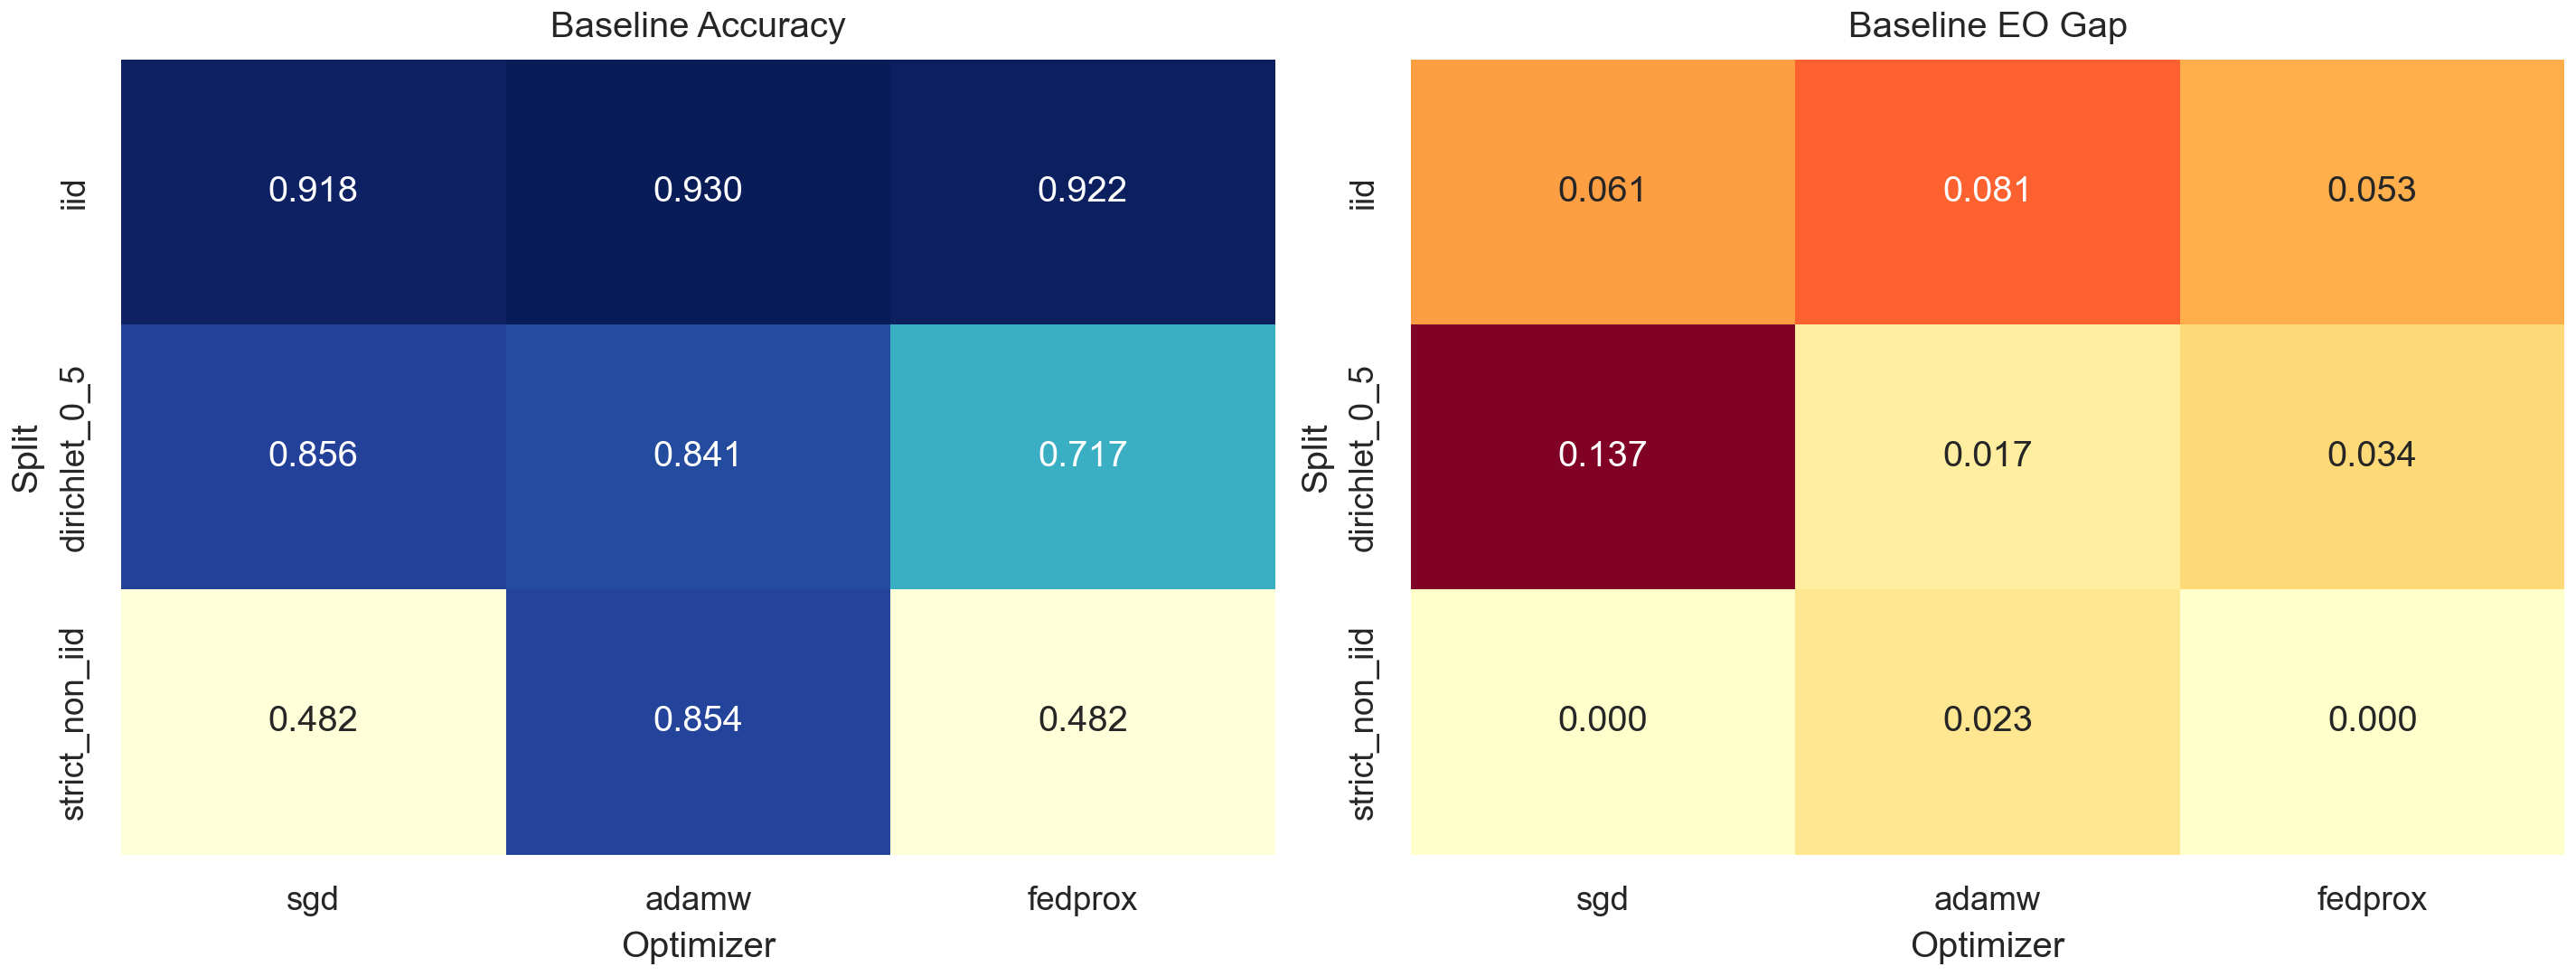
\includegraphics[width=0.95\linewidth]{figures/fig_baseline_heatmaps.png}
  \caption{Baseline heatmaps for accuracy (left) and EO gap (right): AdamW stays stable across splits, while SGD/FedProx fail on strict non-IID.}
  \label{fig:baseline_heatmaps}
\end{figure}

\subsection{Intervention-Only Behavior}

\begin{table}[ht!]
  \caption{Intervention-only averages across split$\times$optimizer.}
  \label{tab:attack_only_summary}
  \centering
  \small
  \begin{tabular}{lcccc}
    \toprule
    \textbf{Intervention} & \textbf{Mean Acc} & \textbf{Mean DP} & \textbf{Mean EO} & \textbf{$\Delta$Acc vs matched baseline} \\
    \midrule
    I$_1$ (A$_1$) & 0.7592 & 0.0155 & 0.0276 & -0.0188 \\
    I$_2$ (A$_2$) & 0.7688 & 0.0238 & 0.0431 & -0.0093 \\
    I$_3$ (A$_3$) & 0.7222 & 0.0151 & 0.0339 & -0.0558 \\
    I$_4$ (A$_4$) & 0.6281 & 0.0279 & 0.0433 & -0.1500 \\
    I$_5$ (A$_5$) & 0.6833 & 0.0227 & 0.0428 & -0.0948 \\
    \bottomrule
  \end{tabular}
\end{table}

I$_4$ is the most disruptive intervention in mean accuracy, while I$_1$/I$_2$
retain higher utility. Fairness changes should be interpreted jointly
with utility, since low EO can coincide with near-degenerate accuracy
on hard splits.

\begin{figure}[t!]
  \centering
  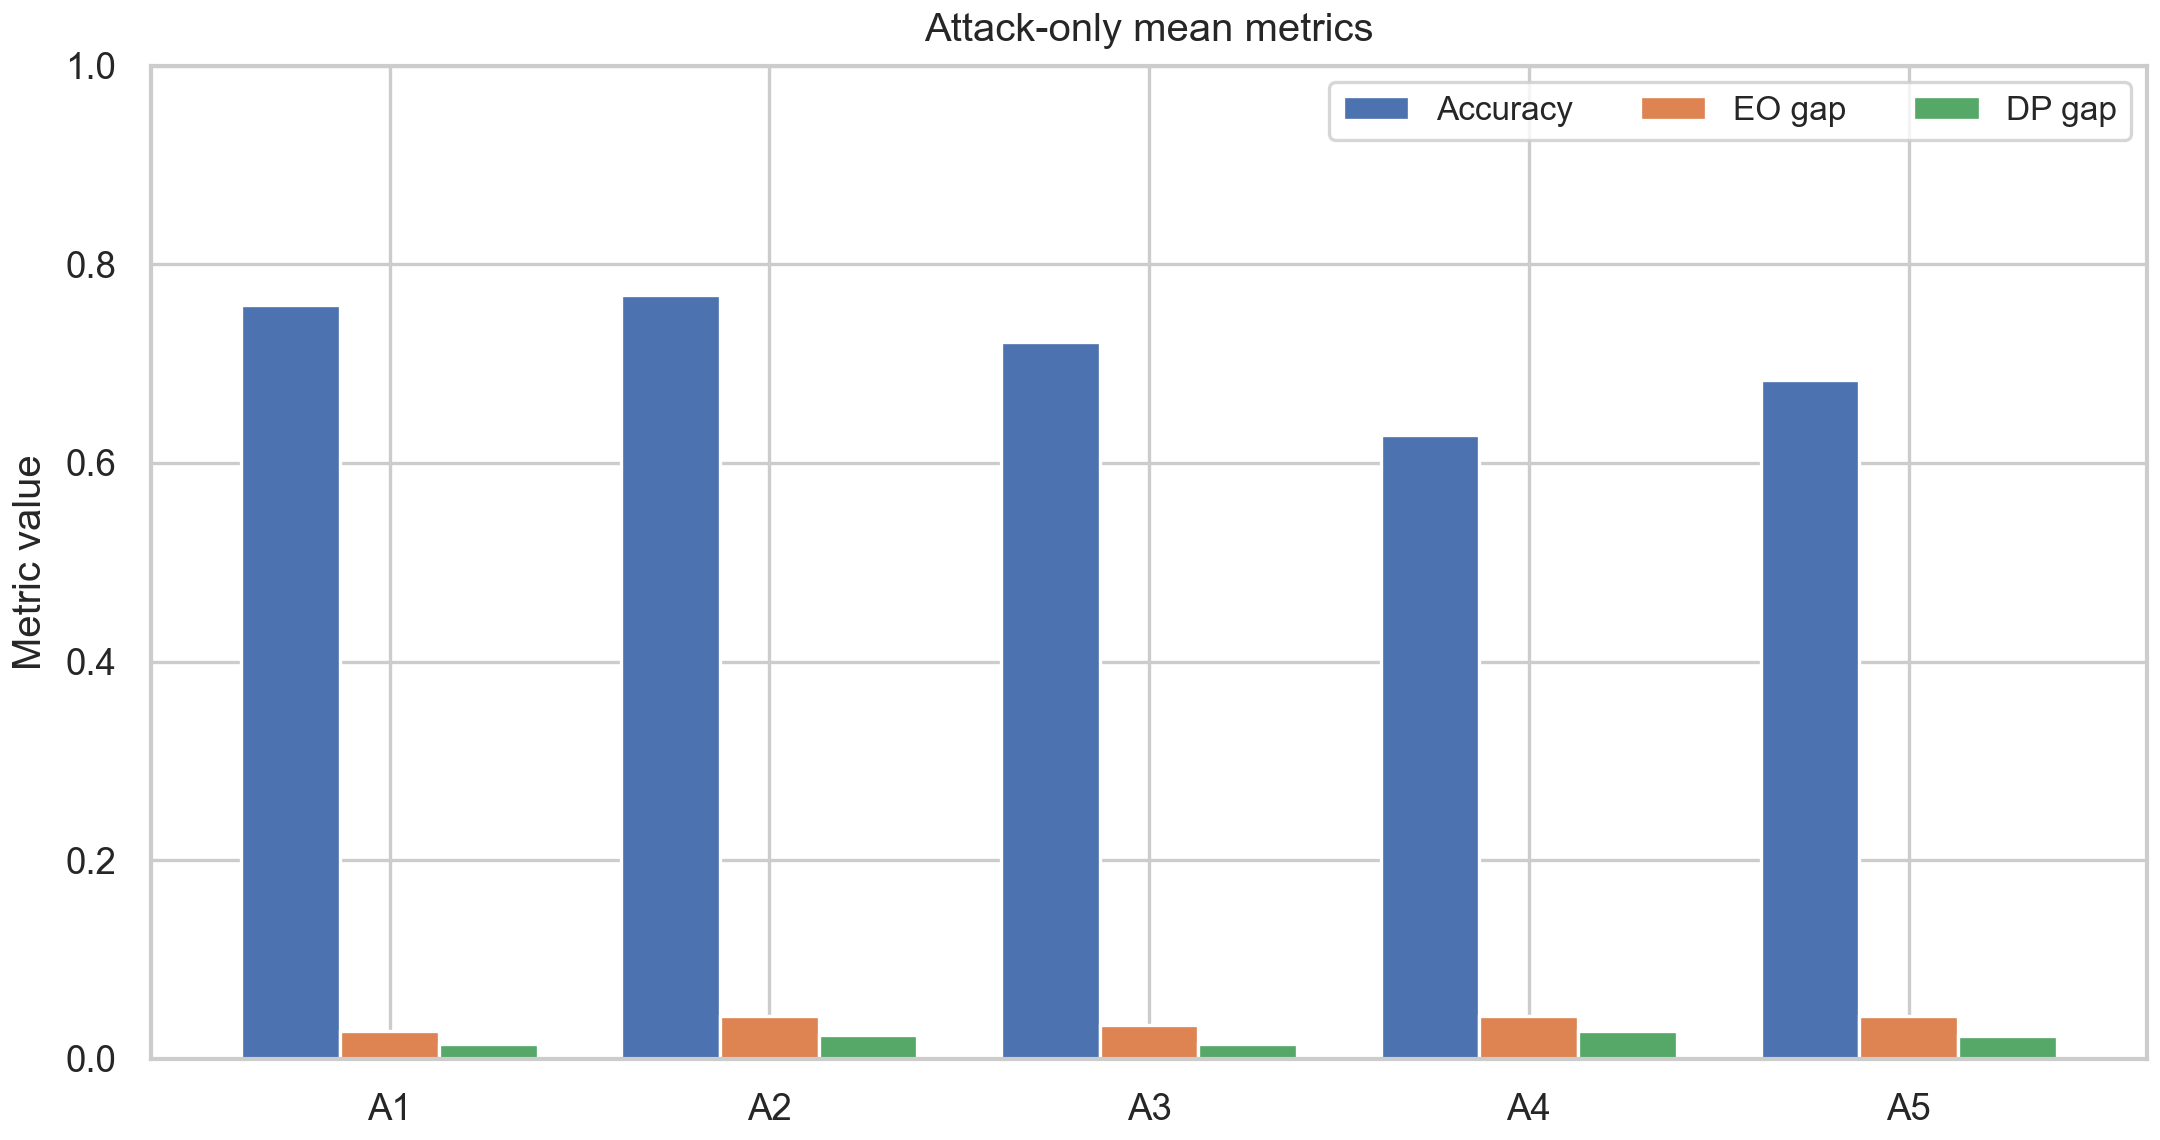
\includegraphics[width=0.75\linewidth]{figures/fig_attack_only_summary.png}
  \caption{Intervention-only means by family: representation-level interventions (I$_4$, I$_5$) incur the largest utility cost.}
  \label{fig:attack_only_summary}
\end{figure}

\subsection{Protocol Effects and Metric Disagreement}

\begin{table}[ht!]
  \caption{Protocol-wise averages over all compatible interventions, splits, and optimizers.}
  \label{tab:defense_summary}
  \centering
  \small
  \begin{tabular}{lcccc}
    \toprule
    \textbf{Protocol} & \textbf{Mean Acc} & \textbf{Mean DP} & \textbf{Mean EO} & \textbf{$\Delta$Acc vs intervention-only} \\
    \midrule
    P$_1$ (D$_1$) & 0.5529 & 0.0472 & 0.0613 & -0.1971 \\
    P$_2$ (D$_2$) & 0.5643 & 0.0500 & 0.0671 & -0.1858 \\
    P$_3$ (D$_3$) & 0.5619 & 0.0546 & 0.0744 & -0.1504 \\
    P$_4$ (D$_4$) & 0.5758 & 0.0682 & 0.0879 & -0.0799 \\
    P$_5$ (D$_5$) & 0.5481 & 0.0511 & 0.0711 & -0.1076 \\
    \bottomrule
  \end{tabular}
\end{table}

No protocol dominates globally.
P$_4$ provides the highest mean accuracy but at the highest fairness
gap; P$_1$ provides the best mean EO gap but with the largest utility
degradation.
DP and EO are not interchangeable in this matrix: in 15 of 45
intervention$\times$split$\times$optimizer cells, the protocol that
minimizes DP is different from the one that minimizes EO.

\begin{figure}[t!]
  \centering
  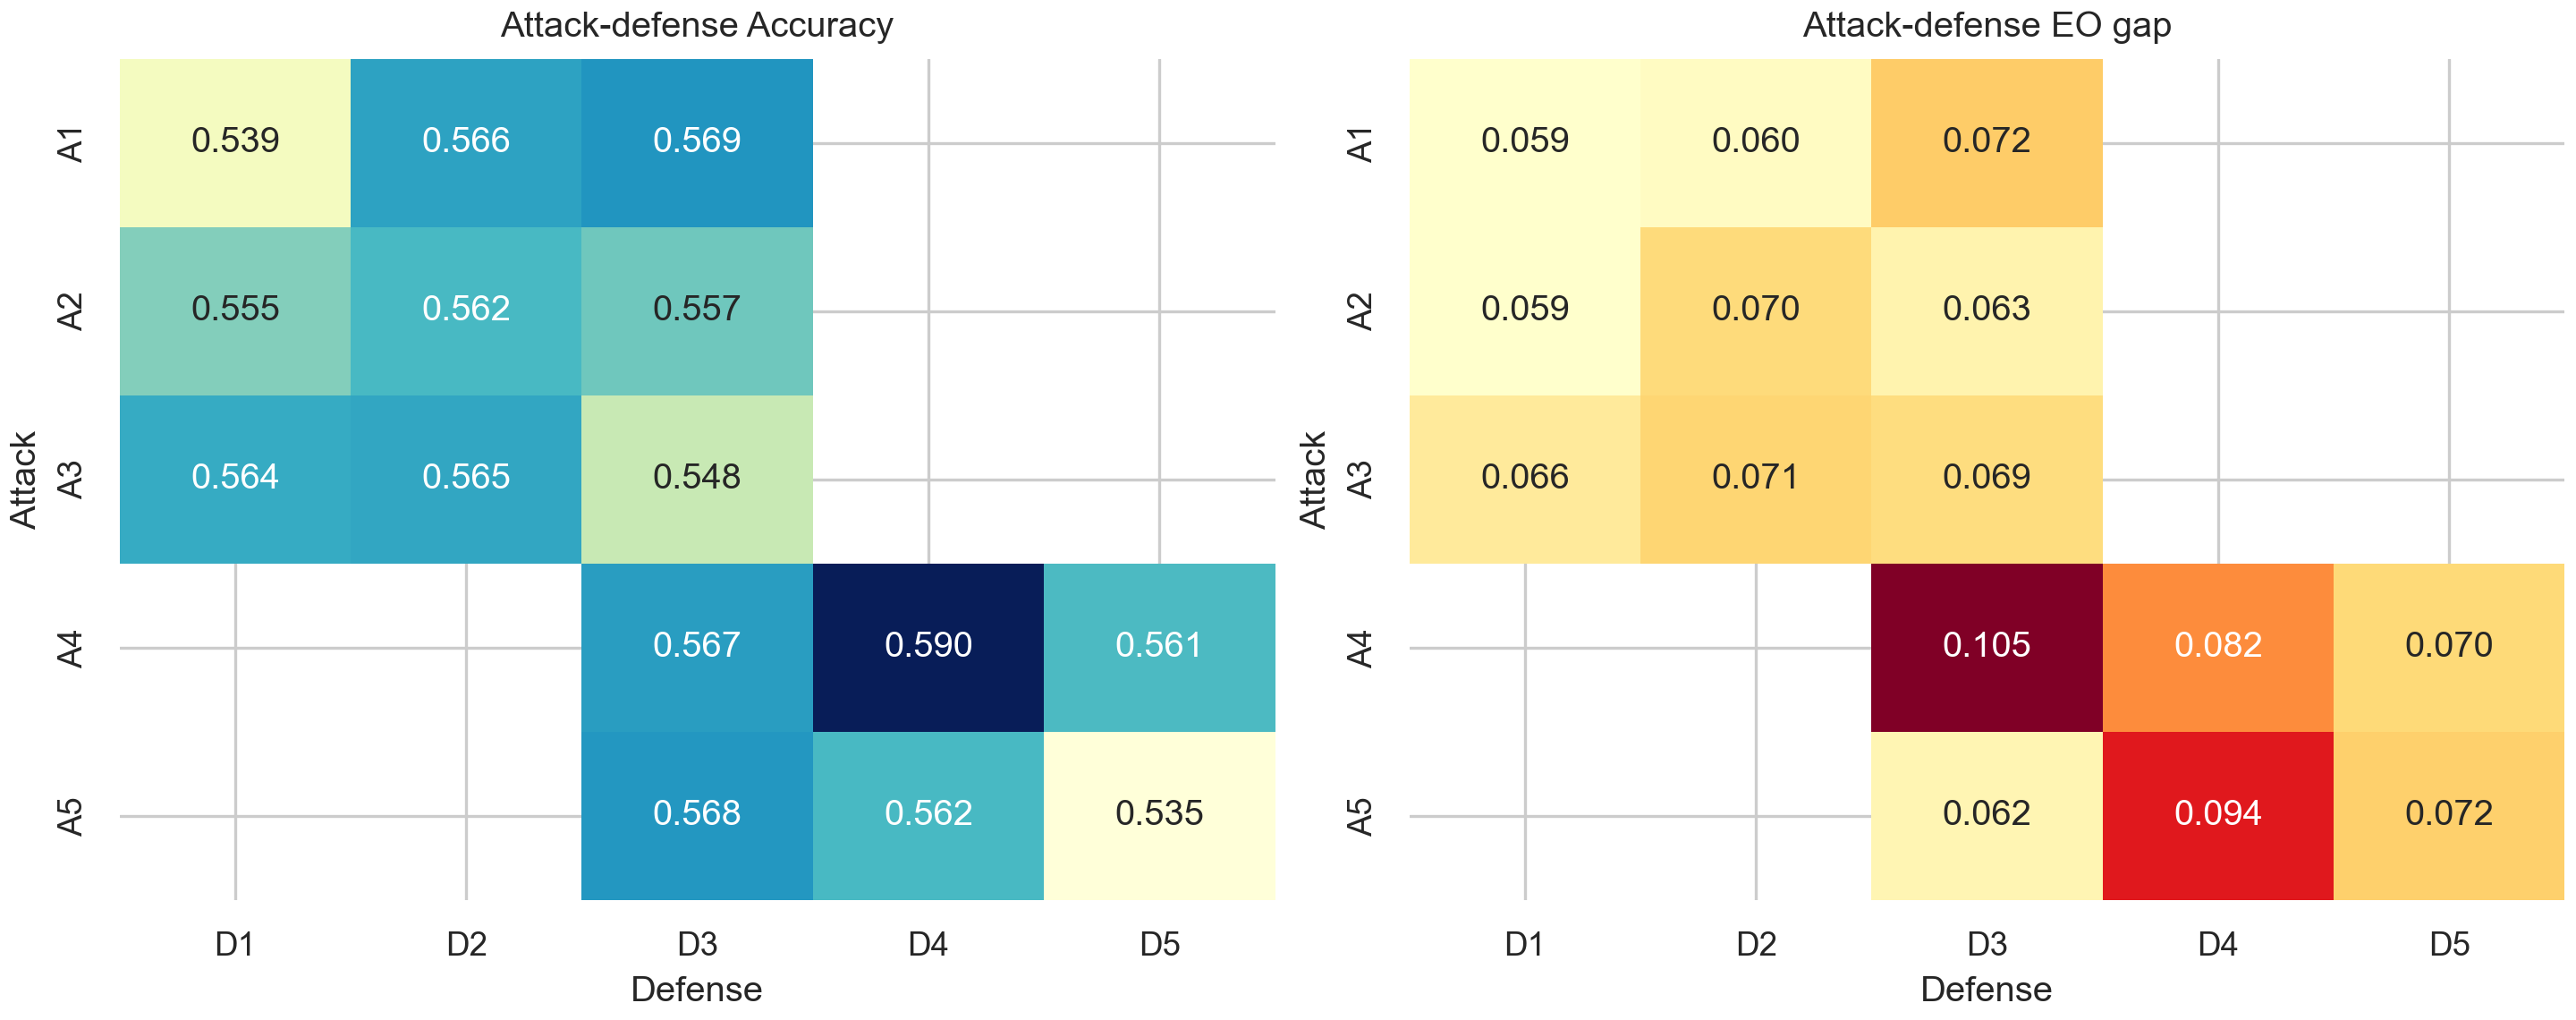
\includegraphics[width=0.95\linewidth]{figures/fig_attack_defense_matrix.png}
  \caption{Intervention-protocol matrix heatmaps: P$_4$ often maximizes accuracy but tends to worsen EO relative to P$_1$.}
  \label{fig:ad_matrix}
\end{figure}

\subsection{Optimizer-Conditional Robustness and Degenerate Regimes}

\begin{table}[ht!]
  \caption{Optimizer means by experimental category.}
  \label{tab:optimizer_robustness}
  \centering
  \small
  \begin{tabular}{llcc}
    \toprule
    \textbf{Category} & \textbf{Optimizer} & \textbf{Mean Acc} & \textbf{Mean EO} \\
    \midrule
    baseline & adamw   & 0.8749 & 0.0402 \\
    baseline & fedprox & 0.7070 & 0.0290 \\
    baseline & sgd     & 0.7523 & 0.0658 \\
    \midrule
    intervention\_only & adamw   & 0.7687 & 0.0511 \\
    intervention\_only & fedprox & 0.6931 & 0.0393 \\
    intervention\_only & sgd     & 0.6752 & 0.0240 \\
    \midrule
    intervention\_protocol & adamw   & 0.7730 & 0.0579 \\
    intervention\_protocol & fedprox & 0.4543 & 0.0784 \\
    intervention\_protocol & sgd     & 0.4545 & 0.0788 \\
    \bottomrule
  \end{tabular}
\end{table}

The dominant empirical pattern is optimizer-conditional robustness:
in intervention+protocol runs, AdamW substantially outperforms
SGD/FedProx.
Therefore, conclusions about ``effective protocols'' are invalid unless
optimizer is explicitly controlled.

\begin{table}[ht!]
  \caption{Effect of removing degenerate runs (Acc $\leq$ 0.55) from intervention+protocol aggregates.}
  \label{tab:degenerate_filter}
  \centering
  \small
  \begin{tabular}{llccc}
    \toprule
    \textbf{Subset} & \textbf{Optimizer} & \textbf{Mean Acc} & \textbf{Mean EO} & \textbf{N runs} \\
    \midrule
    All runs & adamw & 0.7730 & 0.0579 & 45 \\
    All runs & sgd & 0.4545 & 0.0788 & 45 \\
    All runs & fedprox & 0.4543 & 0.0784 & 45 \\
    \midrule
    Acc $>$ 0.55 only & adamw & 0.8576 & 0.0676 & 34 \\
    Acc $>$ 0.55 only & sgd & -- & -- & 0 \\
    Acc $>$ 0.55 only & fedprox & -- & -- & 0 \\
    \bottomrule
  \end{tabular}
\end{table}

The low means for SGD/FedProx in Table~\ref{tab:optimizer_robustness}
are therefore largely driven by strict non-IID collapse rather than
competitive low-accuracy equilibria.

\subsection{Pareto Frontier, Round Dynamics, and Split Diagnostics}

\begin{figure}[t!]
  \centering
  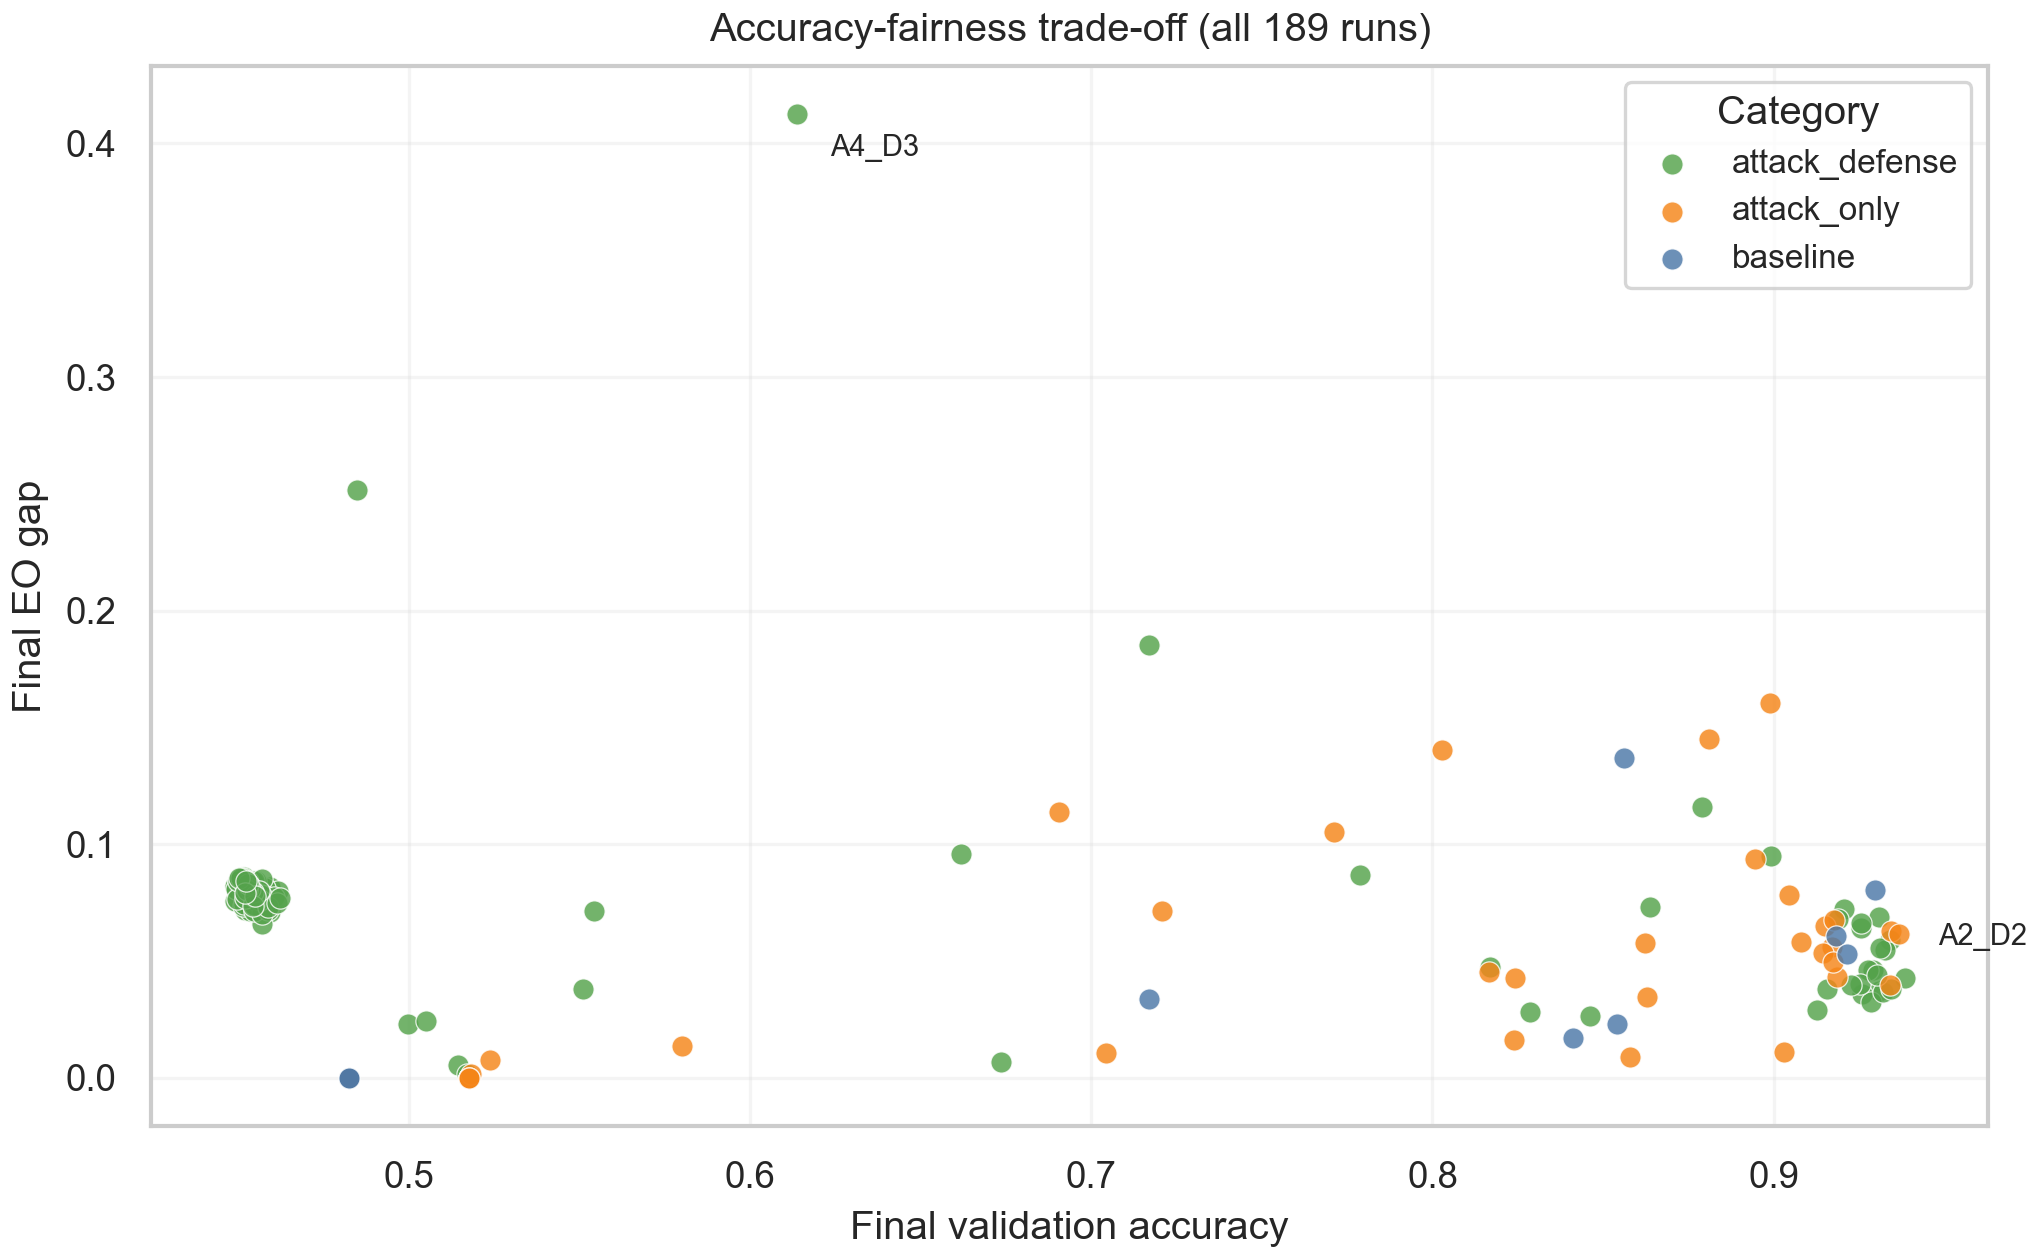
\includegraphics[width=0.78\linewidth]{figures/fig_scatter.png}
  \caption{Accuracy-EO scatter across all 189 runs: the top-accuracy point and largest-EO outlier are both visible and should be interpreted jointly.}
  \label{fig:scatter}
\end{figure}

The best-accuracy run is A$_2$+D$_2$ under IID with AdamW
(accuracy 0.9384, EO 0.0426).
Relative to the matched IID+AdamW baseline (0.9297), this is a
+0.0087 gain, suggesting that some intervention-protocol pairings can
act as regularizers rather than purely harmful perturbations.
The largest EO outlier is A$_4$+D$_3$ under strict non-IID with AdamW
(accuracy 0.6138, EO 0.4126), illustrating that high utility and
extreme fairness disparity can co-occur.

\begin{figure}[t!]
  \centering
  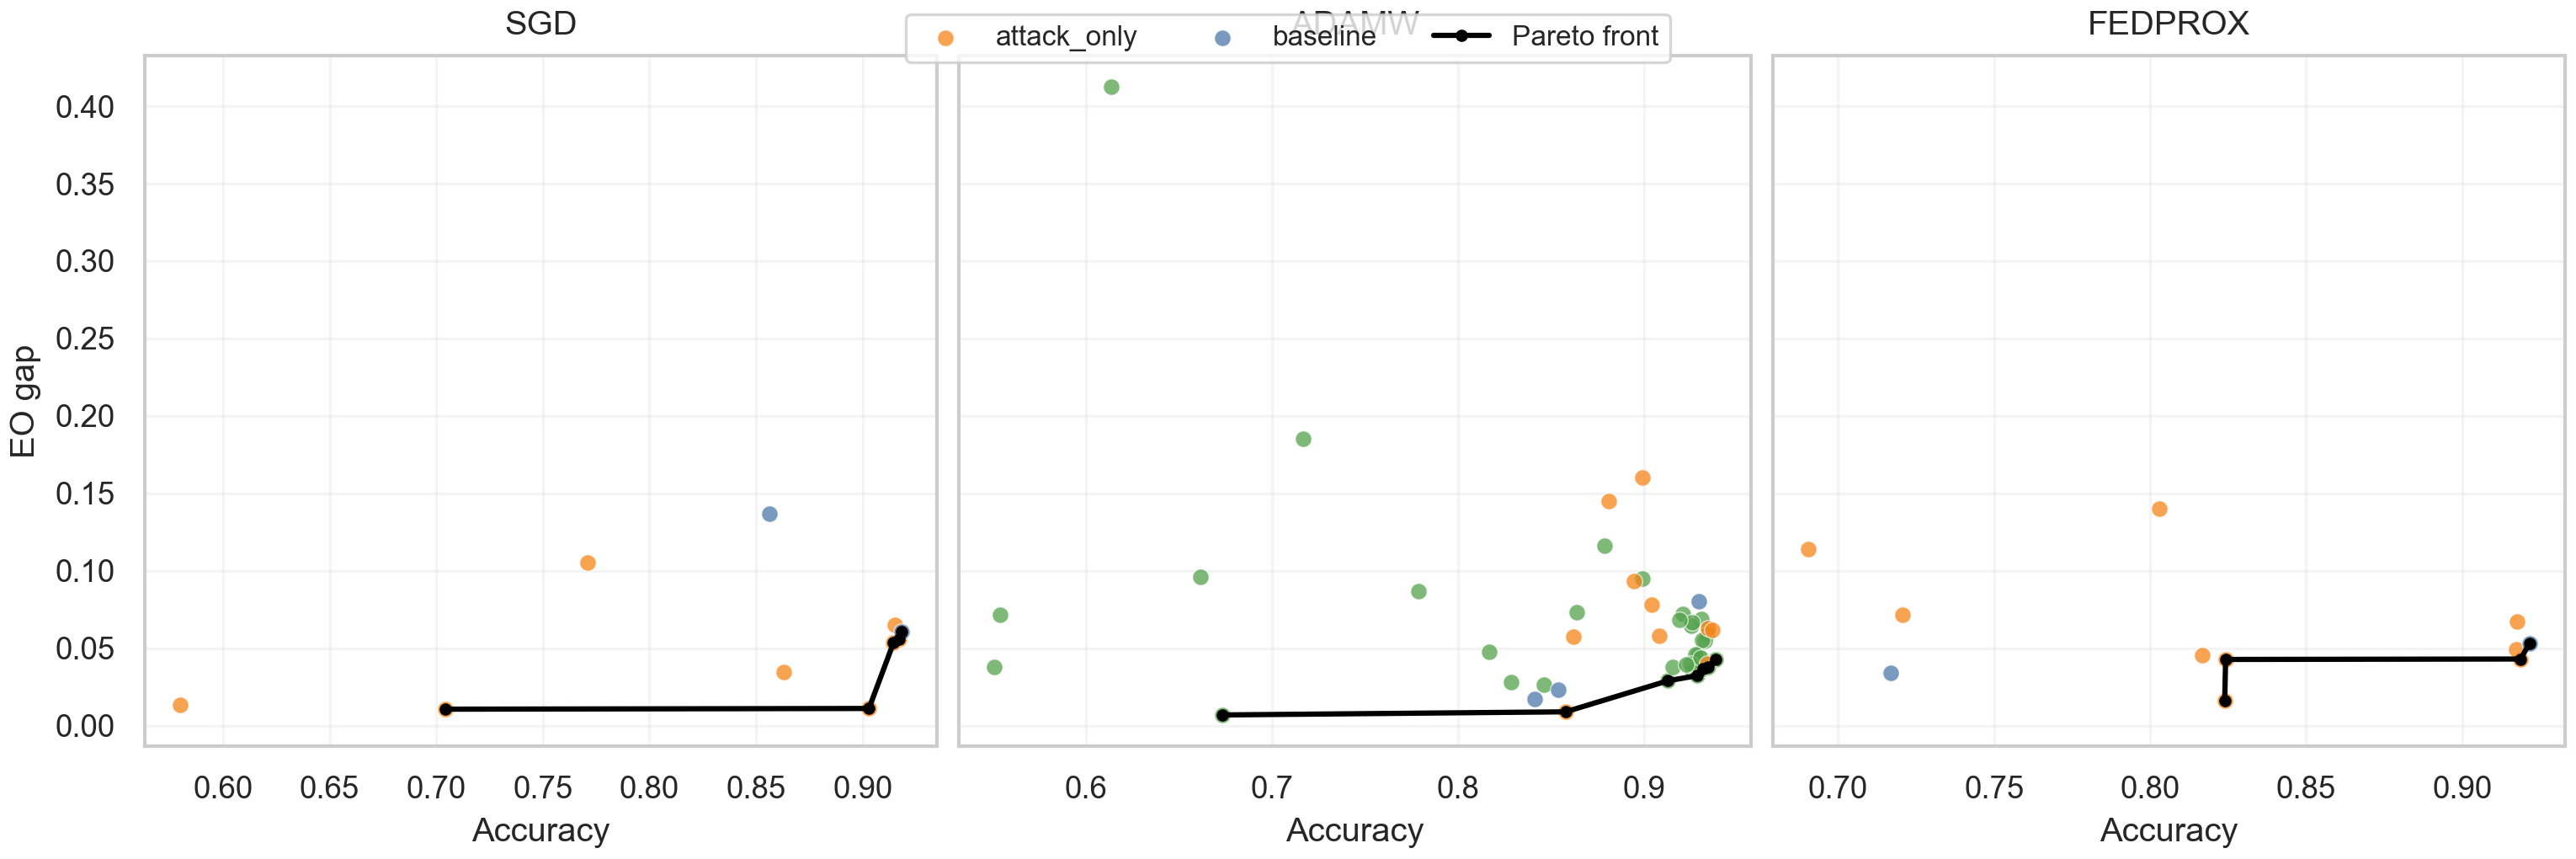
\includegraphics[width=0.98\linewidth]{figures/fig_optimizer_pareto.png}
  \caption{Optimizer-specific Pareto fronts after excluding degenerate runs (Acc $\leq$ 0.55): AdamW forms the strongest frontier across most of the practical operating range.}
  \label{fig:optimizer_pareto}
\end{figure}

\begin{table}[ht!]
  \caption{Convergence proxy by split/optimizer: fraction of runs with
  $|\Delta\text{Acc}_{26\rightarrow30}| < 0.01$.}
  \label{tab:convergence}
  \centering
  \small
  \begin{tabular}{lccc}
    \toprule
    \textbf{Split} & \textbf{SGD} & \textbf{AdamW} & \textbf{FedProx} \\
    \midrule
    iid & 0.905 & 0.952 & 0.952 \\
    dirichlet\_0\_5 & 0.762 & 0.286 & 0.619 \\
    strict\_non\_iid & 0.857 & 0.429 & 0.905 \\
    \bottomrule
  \end{tabular}
\end{table}

\begin{figure}[t!]
  \centering
  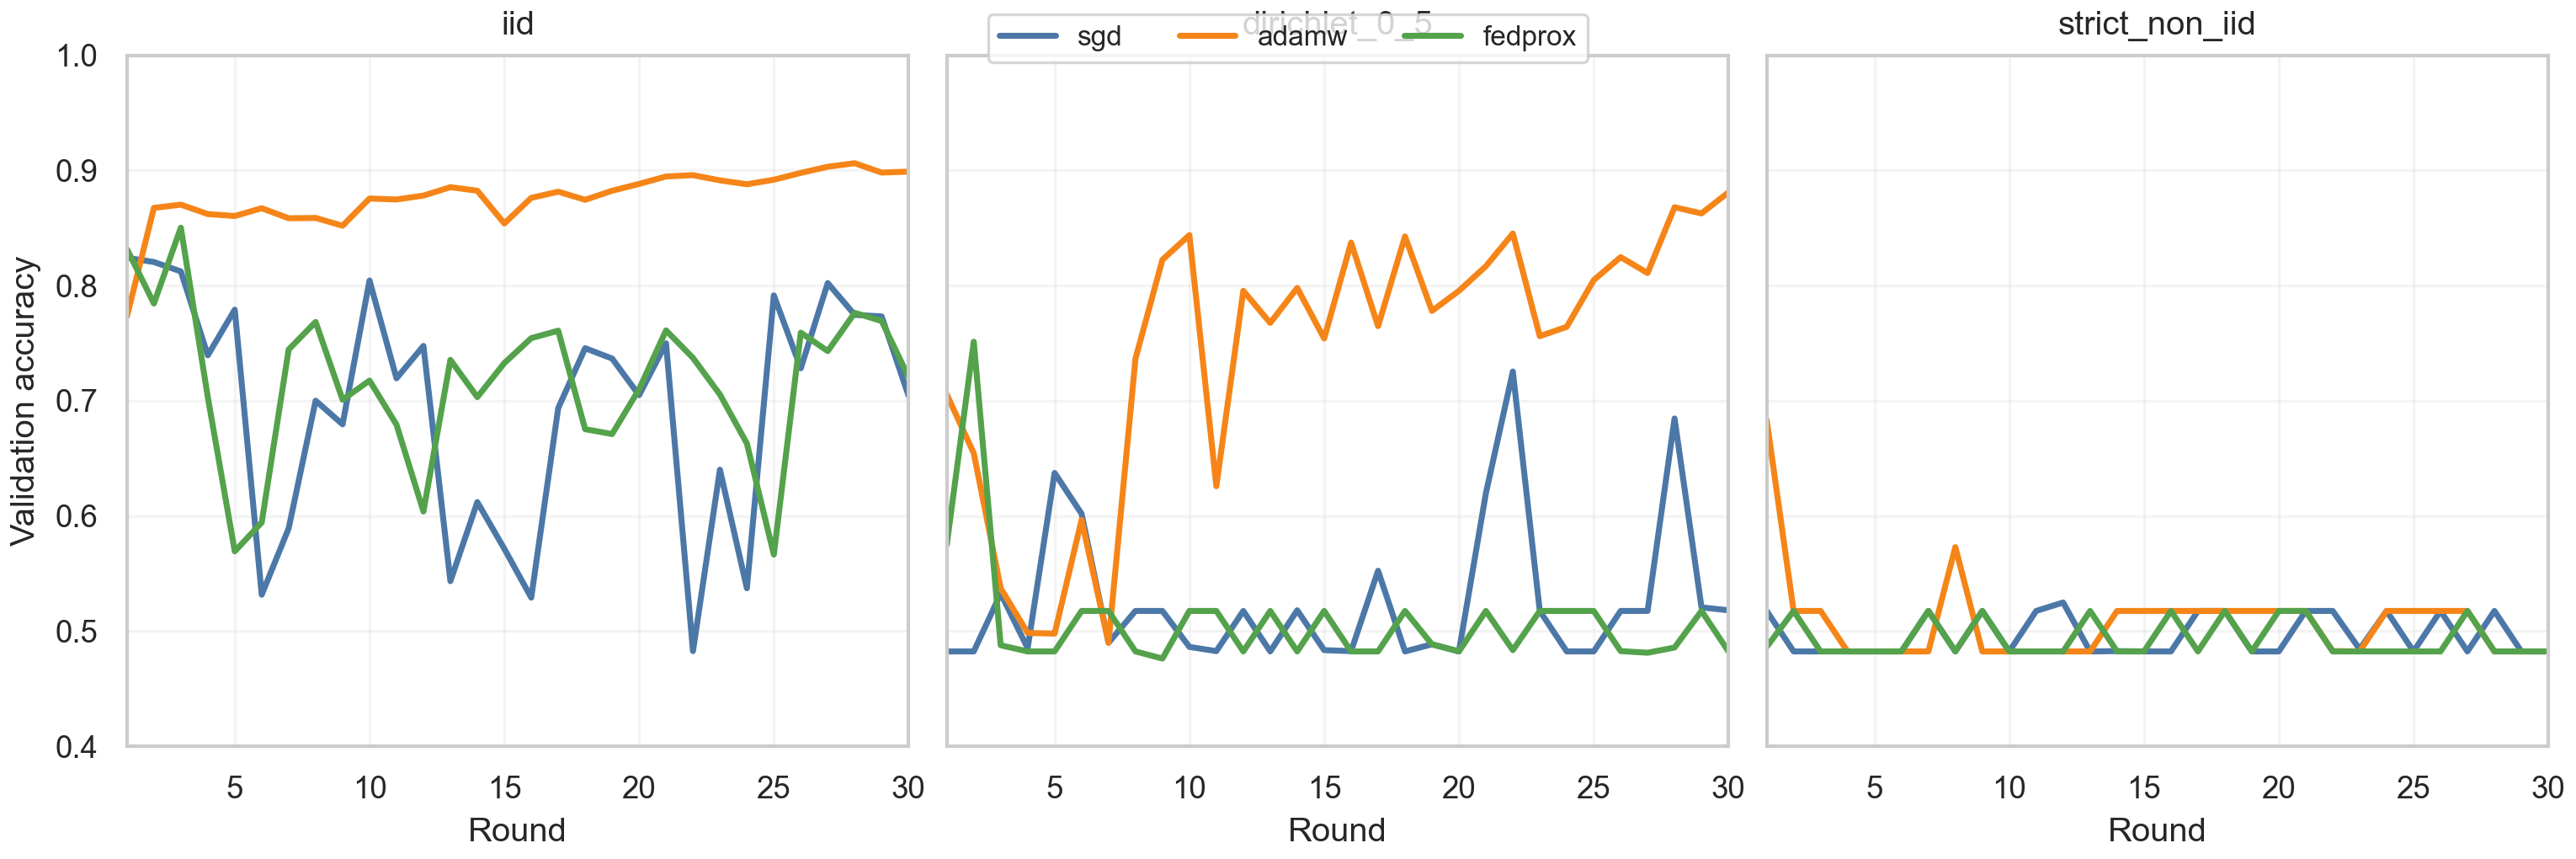
\includegraphics[width=0.98\linewidth]{figures/fig_a4_dynamics.png}
  \caption{Round-wise dynamics for I$_4$ (A$_4$): collapse behavior depends strongly on split and optimizer, and several non-IID cells remain non-stationary at 30 rounds.}
  \label{fig:a4_dynamics}
\end{figure}

\begin{figure}[t!]
  \centering
  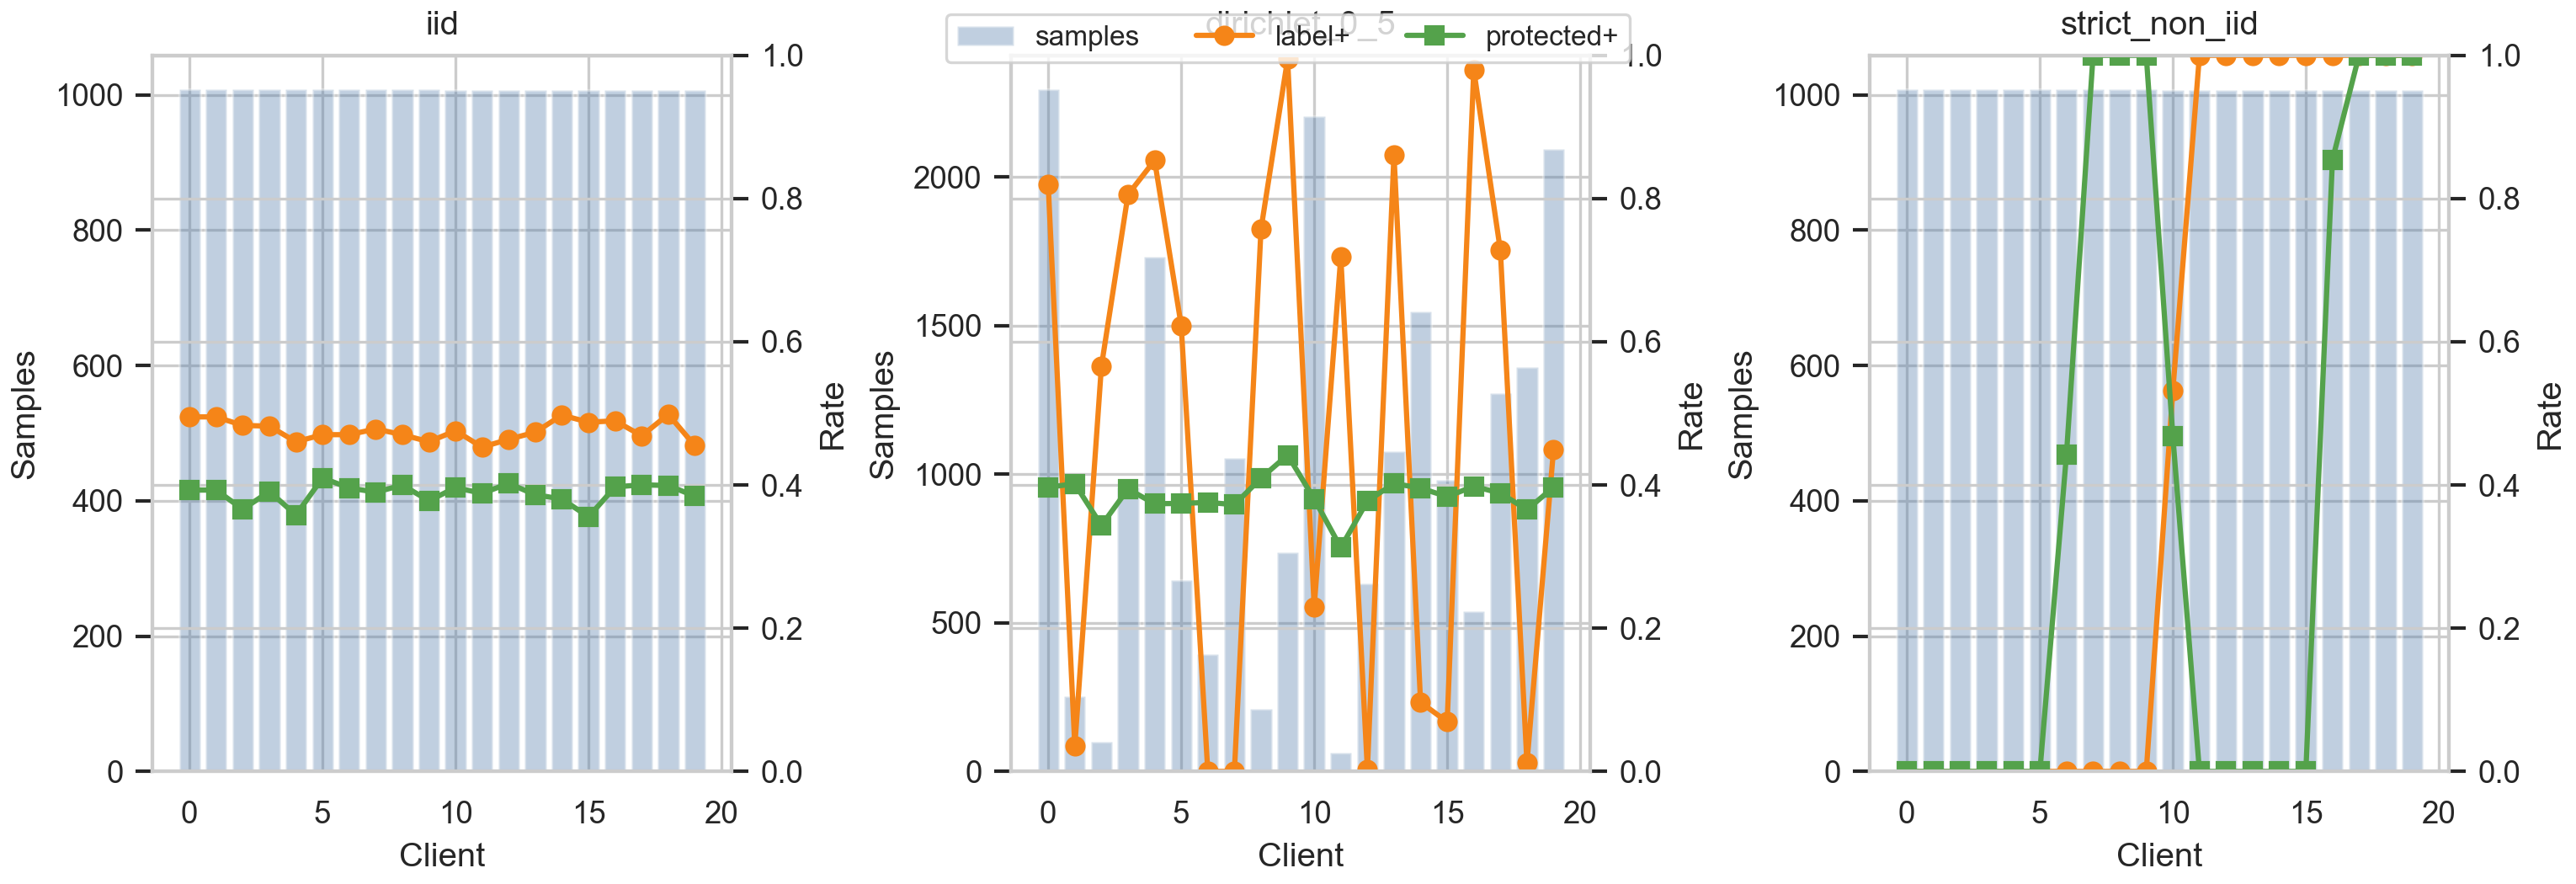
\includegraphics[width=0.95\linewidth]{figures/fig_data_distribution.png}
  \caption{Per-client sample and rate diagnostics: strict non-IID reaches extreme 0/1 label and protected-group regimes, explaining frequent degenerate operating points.}
  \label{fig:distributions}
\end{figure}

Split statistics explain this behavior:
IID is tightly balanced (samples/client 1007--1008),
Dirichlet exhibits severe sample skew (64--2295), and strict non-IID
has extreme label/protected rates (0 to 1).
Under strict non-IID, 54/63 runs fall in 0.45--0.55 accuracy,
and 23/63 runs report EO gap 0.0, indicating frequent near-degenerate
operating points.

% ─────────────────────────────────────────────────────────────────────────────
\section{Discussion}
\label{sec:discussion}
% ─────────────────────────────────────────────────────────────────────────────

\paragraph{Effect of heterogeneity.}
Performance degrades with split severity.
Across all runs, mean accuracy is 0.6874 (IID), 0.6413 (Dirichlet), and
0.4926 (strict non-IID).
The strict non-IID setting frequently enters near-degenerate regimes,
which can artificially deflate fairness gaps without meaningful utility.

\paragraph{Intervention complexity at scale.}
I$_4$ and I$_5$ are the most utility-disruptive interventions on average,
with matched-baseline drops of -0.1500 and -0.0948.
In contrast, I$_1$ and I$_2$ preserve substantially more accuracy.
This indicates that stronger intervention complexity does not translate
into uniformly better accuracy-fairness operating points.

\paragraph{Protocol effectiveness.}
No protocol is globally dominant.
P$_4$ yields the best mean accuracy (0.5758) but the worst mean EO gap
(0.0879), while P$_1$ yields the best mean EO gap (0.0613) at lower
mean accuracy (0.5529).
Hence, protocol choice should be treated as a policy decision over a
utility-fairness frontier, not as a one-dimensional optimization.

\paragraph{Optimiser sensitivity.}
Optimizer choice is the strongest factor in this benchmark.
In intervention+protocol conditions, AdamW reaches mean accuracy 0.7730,
whereas SGD and FedProx remain near 0.454.
The degenerate-filtered analysis (Table~\ref{tab:degenerate_filter})
shows that this gap is largely a collapse-vs-non-collapse phenomenon.
Therefore, any claim about intervention or protocol effectiveness must be
conditioned on optimizer.

\paragraph{Mechanistic interpretation (hypothesis-level).}
The optimizer gap is consistent with adaptive-step-size stabilization:
AdamW appears more resilient to intervention-induced gradient
distortions than SGD/FedProx in high-heterogeneity regimes.
Our current evidence is empirical rather than causal; targeted ablations
separating adaptation, momentum, and weight decay are required before
making mechanistic claims.

\paragraph{Framing boundary.}
This paper analyzes \emph{benign unilateral fairness interventions}, not
malicious Byzantine attacks.
We keep legacy A/D labels for reproducibility with artifacts, but the
appropriate interpretation is intervention strategies and server
auditing/stabilization protocols.

\paragraph{Limitations.}
\begin{enumerate}[leftmargin=1.5em,itemsep=0pt]
  \item The study is single-dataset (UTKFace); cross-dataset
    generalization remains unverified.
  \item The submitted full profile uses one seed, so variance
    estimation is limited and should be extended in future work.
  \item External fairness FL baselines (FairFed, Ditto, AFL, q-FedAvg)
    are not yet included, so cross-method ranking claims are out of
    scope for this draft.
  \item No centralized oracle baseline is reported, so FL-vs-centralized
    fairness gaps are not isolated.
  \item The protected attribute is a binary race proxy
    (\texttt{race\_bin}), which does not capture intersectional
    fairness structure.
  \item Hyperparameter sensitivity is not yet mapped (e.g., strength,
    clipping, and threshold schedules), so rank ordering may shift
    outside the tested setting.
  \item Strict non-IID frequently produces near-degenerate accuracy,
    complicating interpretation of very low fairness gaps.
  \item We do not model client incentives formally, so when and why
    clients would adopt these interventions in practice remains open.
\end{enumerate}

% ─────────────────────────────────────────────────────────────────────────────
\section{Conclusion}
\label{sec:conclusion}
% ─────────────────────────────────────────────────────────────────────────────

We presented a controlled empirical study of client-side fairness
interventions and server auditing protocols in federated learning.
Our full 189-configuration benchmark over three split regimes and
three optimizers shows that optimizer choice dominates
intervention-protocol outcomes: AdamW remains robust under
intervention pressure, while SGD/FedProx often collapse in
intervention+protocol settings.
We also show that no protocol is universally optimal, with clear
trade-offs between utility and fairness metrics.
These findings motivate optimizer-aware fairness governance in FL.
The next experimental milestone is a multi-seed, external-baseline,
and sensitivity-complete benchmark to convert these descriptive trends
into statistically robust comparative conclusions.

% ─────────────────────────────────────────────────────────────────────────────
%  REFERENCES
% ─────────────────────────────────────────────────────────────────────────────
% ─────────────────────────────────────────────────────────────────────────────
%  APPENDIX
% ─────────────────────────────────────────────────────────────────────────────
\appendix

\section{Extended Experimental Details}
\label{app:details}

\subsection{UTKFace Preprocessing}
UTKFace images are loaded at variable native resolution,
resized to $128\!\times\!128$ via bilinear interpolation, and
normalised channel-wise:
$\mu = [0.485, 0.456, 0.406]$, $\sigma = [0.229, 0.224, 0.225]$.
The pipeline uses deterministic resize+normalize transforms.

\subsection{Client Partitioning Details}

\begin{table}[ht!]
  \caption{Measured client-level data statistics by split (seed 42).}
  \label{tab:partition_stats}
  \centering
  \small
  \begin{tabular}{lcccc}
    \toprule
    \textbf{Split} & \textbf{Samples/client} & \textbf{Sample range} & \textbf{Label+ range} & \textbf{Protected+ range} \\
    \midrule
    iid & $1007.5 \pm 0.5$ & 1007--1008 & 0.4528--0.4985 & 0.3555--0.4097 \\
    dirichlet\_0\_5 & $1007.5 \pm 676.45$ & 64--2295 & 0.0000--0.9946 & 0.3125--0.4417 \\
    strict\_non\_iid & $1007.5 \pm 0.5$ & 1007--1008 & 0.0000--1.0000 & 0.0000--1.0000 \\
    \bottomrule
  \end{tabular}
\end{table}

\subsection{Full Hyperparameter Table}

\begin{table}[ht!]
  \caption{Complete hyperparameter grid used in all experiments.}
  \label{tab:hparams}
  \centering
  \small
  \begin{tabular}{lll}
    \toprule
    \textbf{Parameter} & \textbf{Value(s)} & \textbf{Notes} \\
    \midrule
    Communication rounds $T$ & 30 & Full profile \\
    Clients $K$ & 20 & Total clients \\
    Clients per round & 8 & Partial participation \\
    Local epochs $E$ & 1 & Per selected client \\
    Batch size & 64 & All clients \\
    \texttt{num\_workers} & 4 & DataLoader \\
    Validation split & 0.15 & Hold-out validation \\
    \midrule
    SGD learning rate & $10^{-2}$ & Momentum 0.9 \\
    SGD momentum & $0.9$ & \\
    SGD weight decay & $10^{-4}$ & \\
    AdamW learning rate & $10^{-3}$ & \\
    AdamW $(\beta_1, \beta_2)$ & $(0.9, 0.999)$ & \\
    AdamW weight decay & $10^{-4}$ & \\
    FedProx learning rate & $10^{-2}$ & \\
    FedProx $\mu$ & $10^{-3}$ & Proximal coefficient \\
    \midrule
    Intervention strength & 0.25 & Shared coefficient \\
    Protocol strength & 0.25 & Shared coefficient \\
    Checkpoint period & Every 5 rounds & Resume enabled \\
    Seed list & \{42\} & Single-seed submission run \\
    AMP & Enabled & Mixed precision training \\
    \bottomrule
  \end{tabular}
\end{table}

\subsection{Artifact Files}

The run exports all report-facing artifacts as CSV/JSON:
\begin{itemize}[leftmargin=1.25em,itemsep=0pt]
  \item \texttt{all\_runs\_final.csv}, \texttt{all\_rounds.csv}
  \item \texttt{table2\_baseline.csv}
  \item \texttt{fig1\_fig3\_fig5\_attack\_only.csv}
  \item \texttt{table1\_fig4\_attack\_defense.csv}
  \item \texttt{fig2\_data\_distribution.csv}
  \item \texttt{fig6\_scatter\_source.csv}
\end{itemize}
These files are sufficient to regenerate all tables and figures in this submission.

\end{document}


